\subsection{Resultado - Exercício 3}

Os passos são:
\begin{itemize}[leftmargin=3.5em, itemsep=-.5mm, topsep=0.5mm]
    \item Transformar sin(x) em série.
    \item Aplicar a fórmula do resíduo e definir o tamanho da série
    \item Imprimir a função na forma de série e usando numpy no python
    \item Realizar os testes
    \item Apresentar o código Python e GnuPlot
 \end{itemize}

\newpage

\subsubsection{Transformar $sin(x)$ em série.}
Temos os calculos para escrever $sin(x)$ usando a Série de Taylor.
\begin{figure}[H]
    \centering
    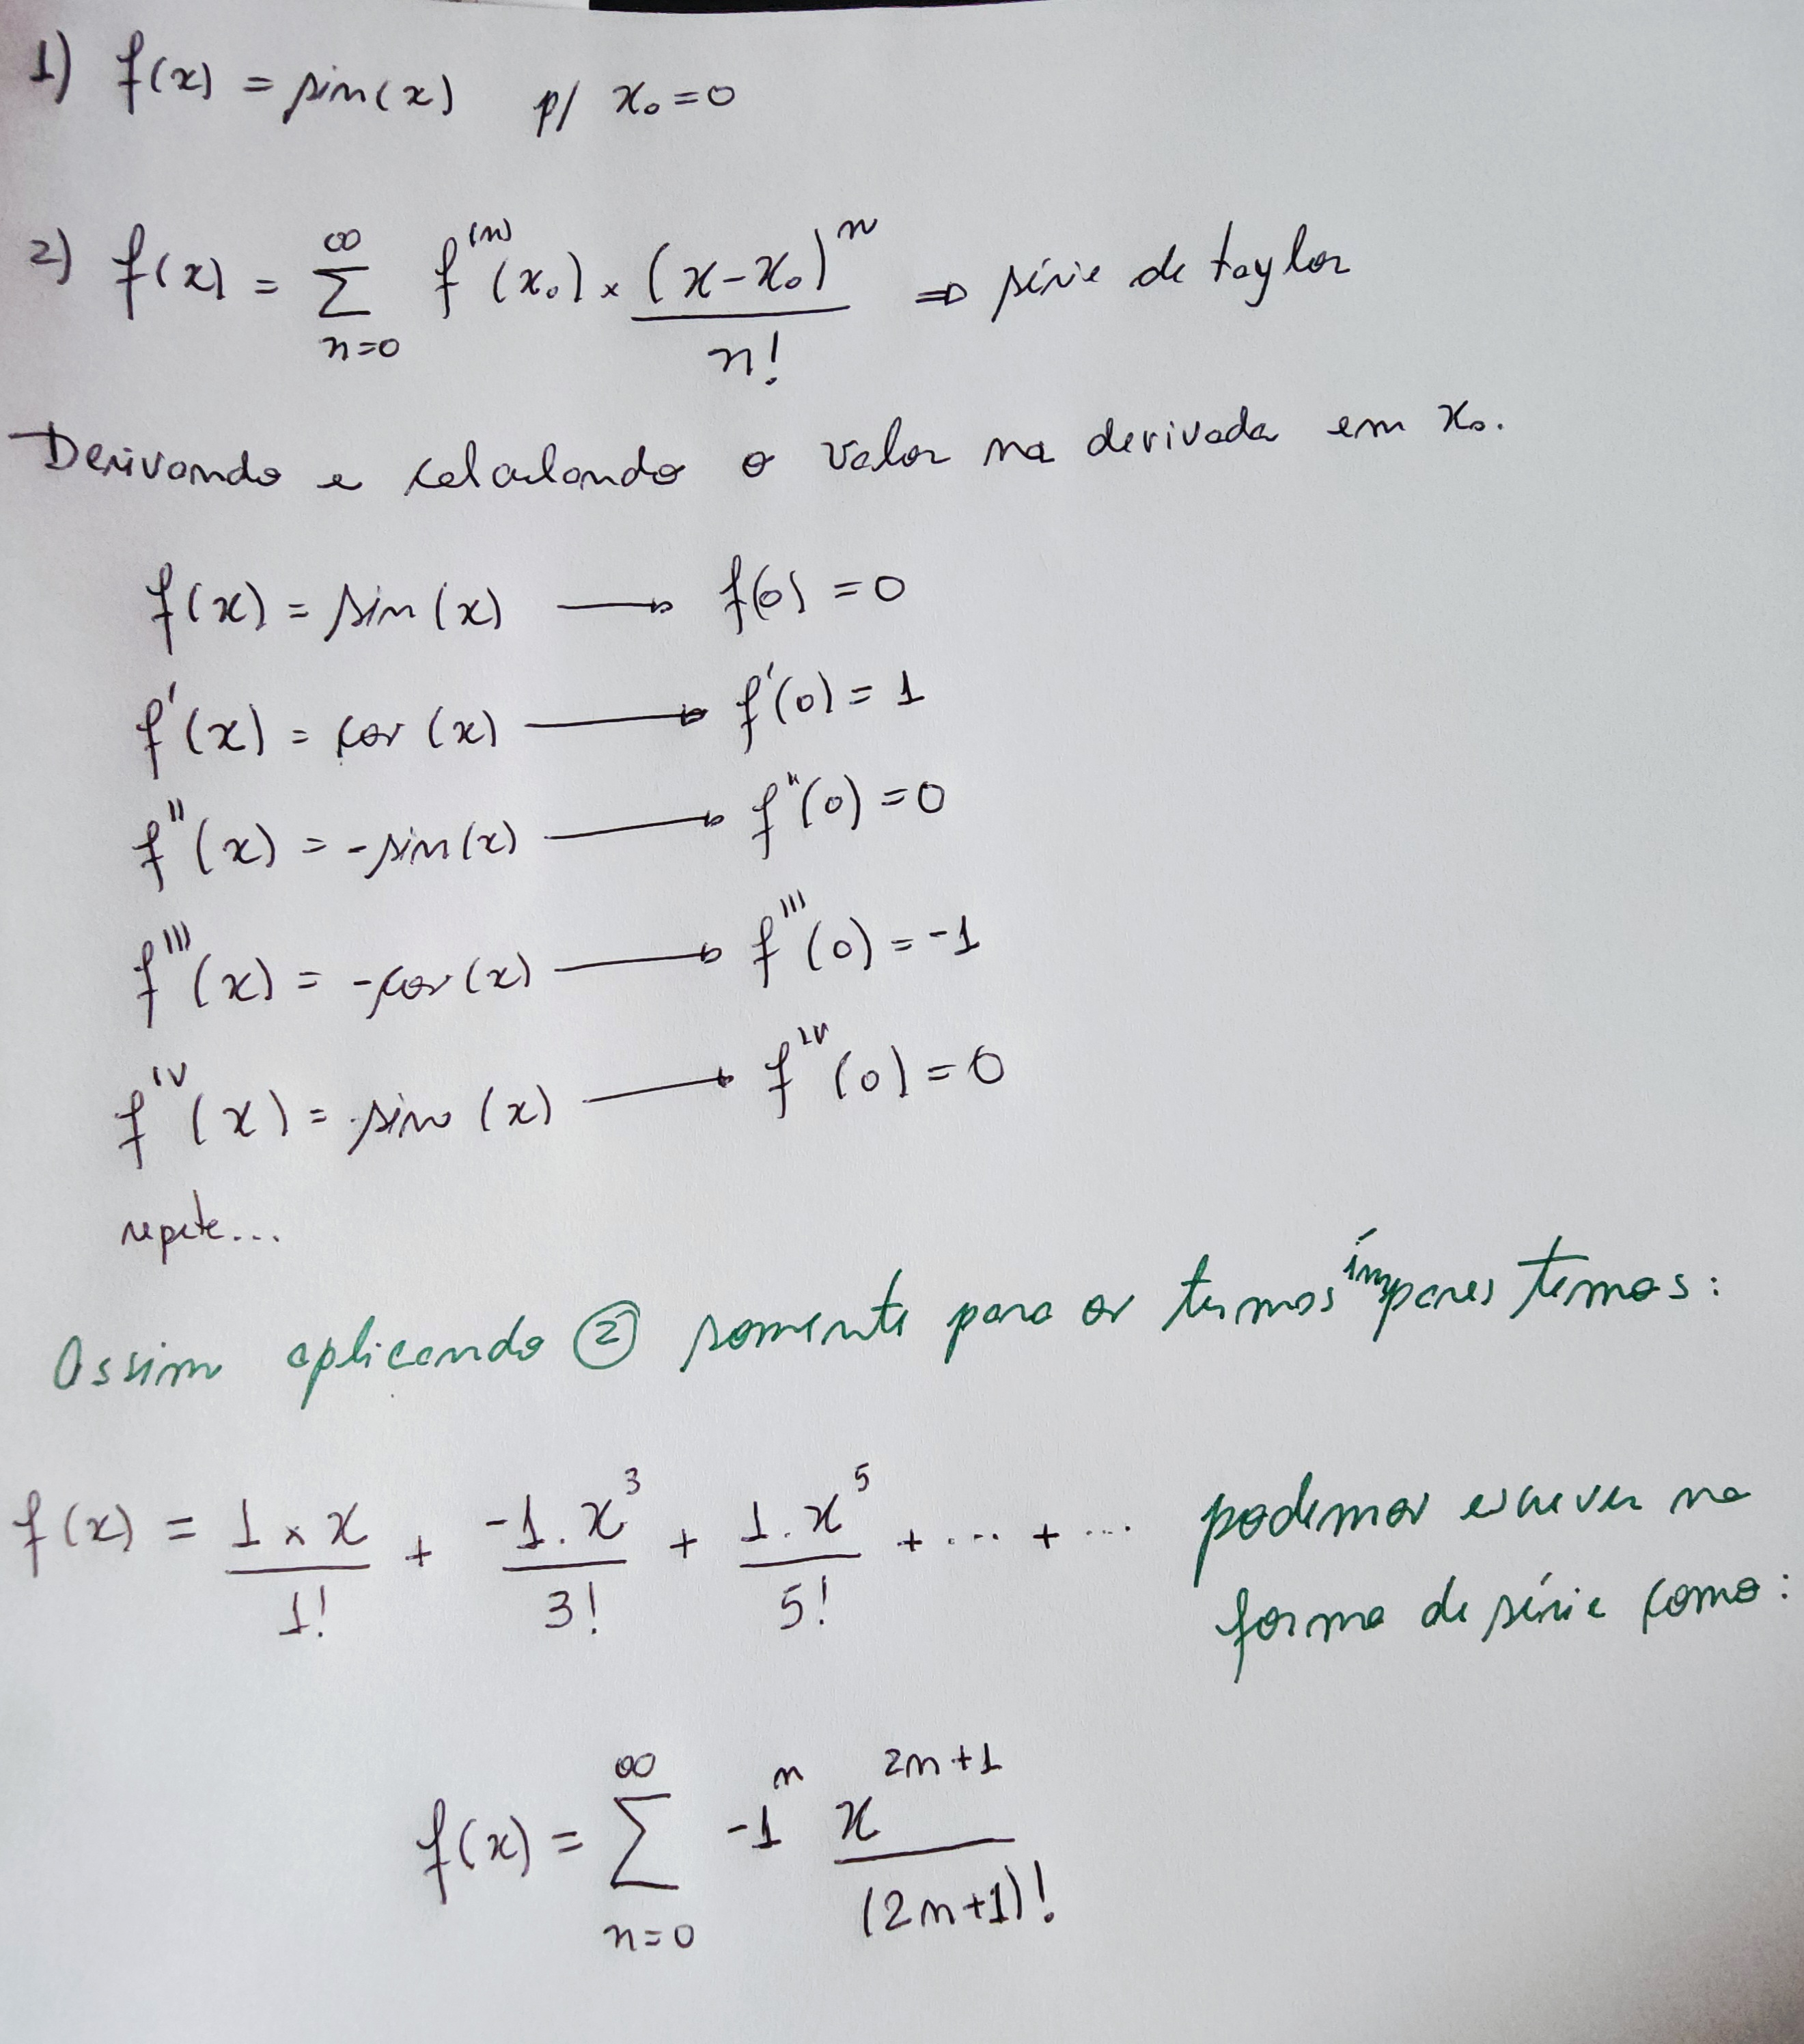
\includegraphics[width=1.0\textwidth]{imagens/exercicio3_parte_1}
    \caption{Escrevendo $sin(x)$ na forma de série entre $0$ e $\pi/2$}
    \label{fig:lista_exercicio3_parte1}
\end{figure}
\newpage

\subsubsection{Aplicar a fórmula do resíduo e definir o tamanho da série}
Aplicando as Equações de resíduo de Taylor e o valor médio para integrais ponderadas temos:
\begin{figure}[H]
    \centering
    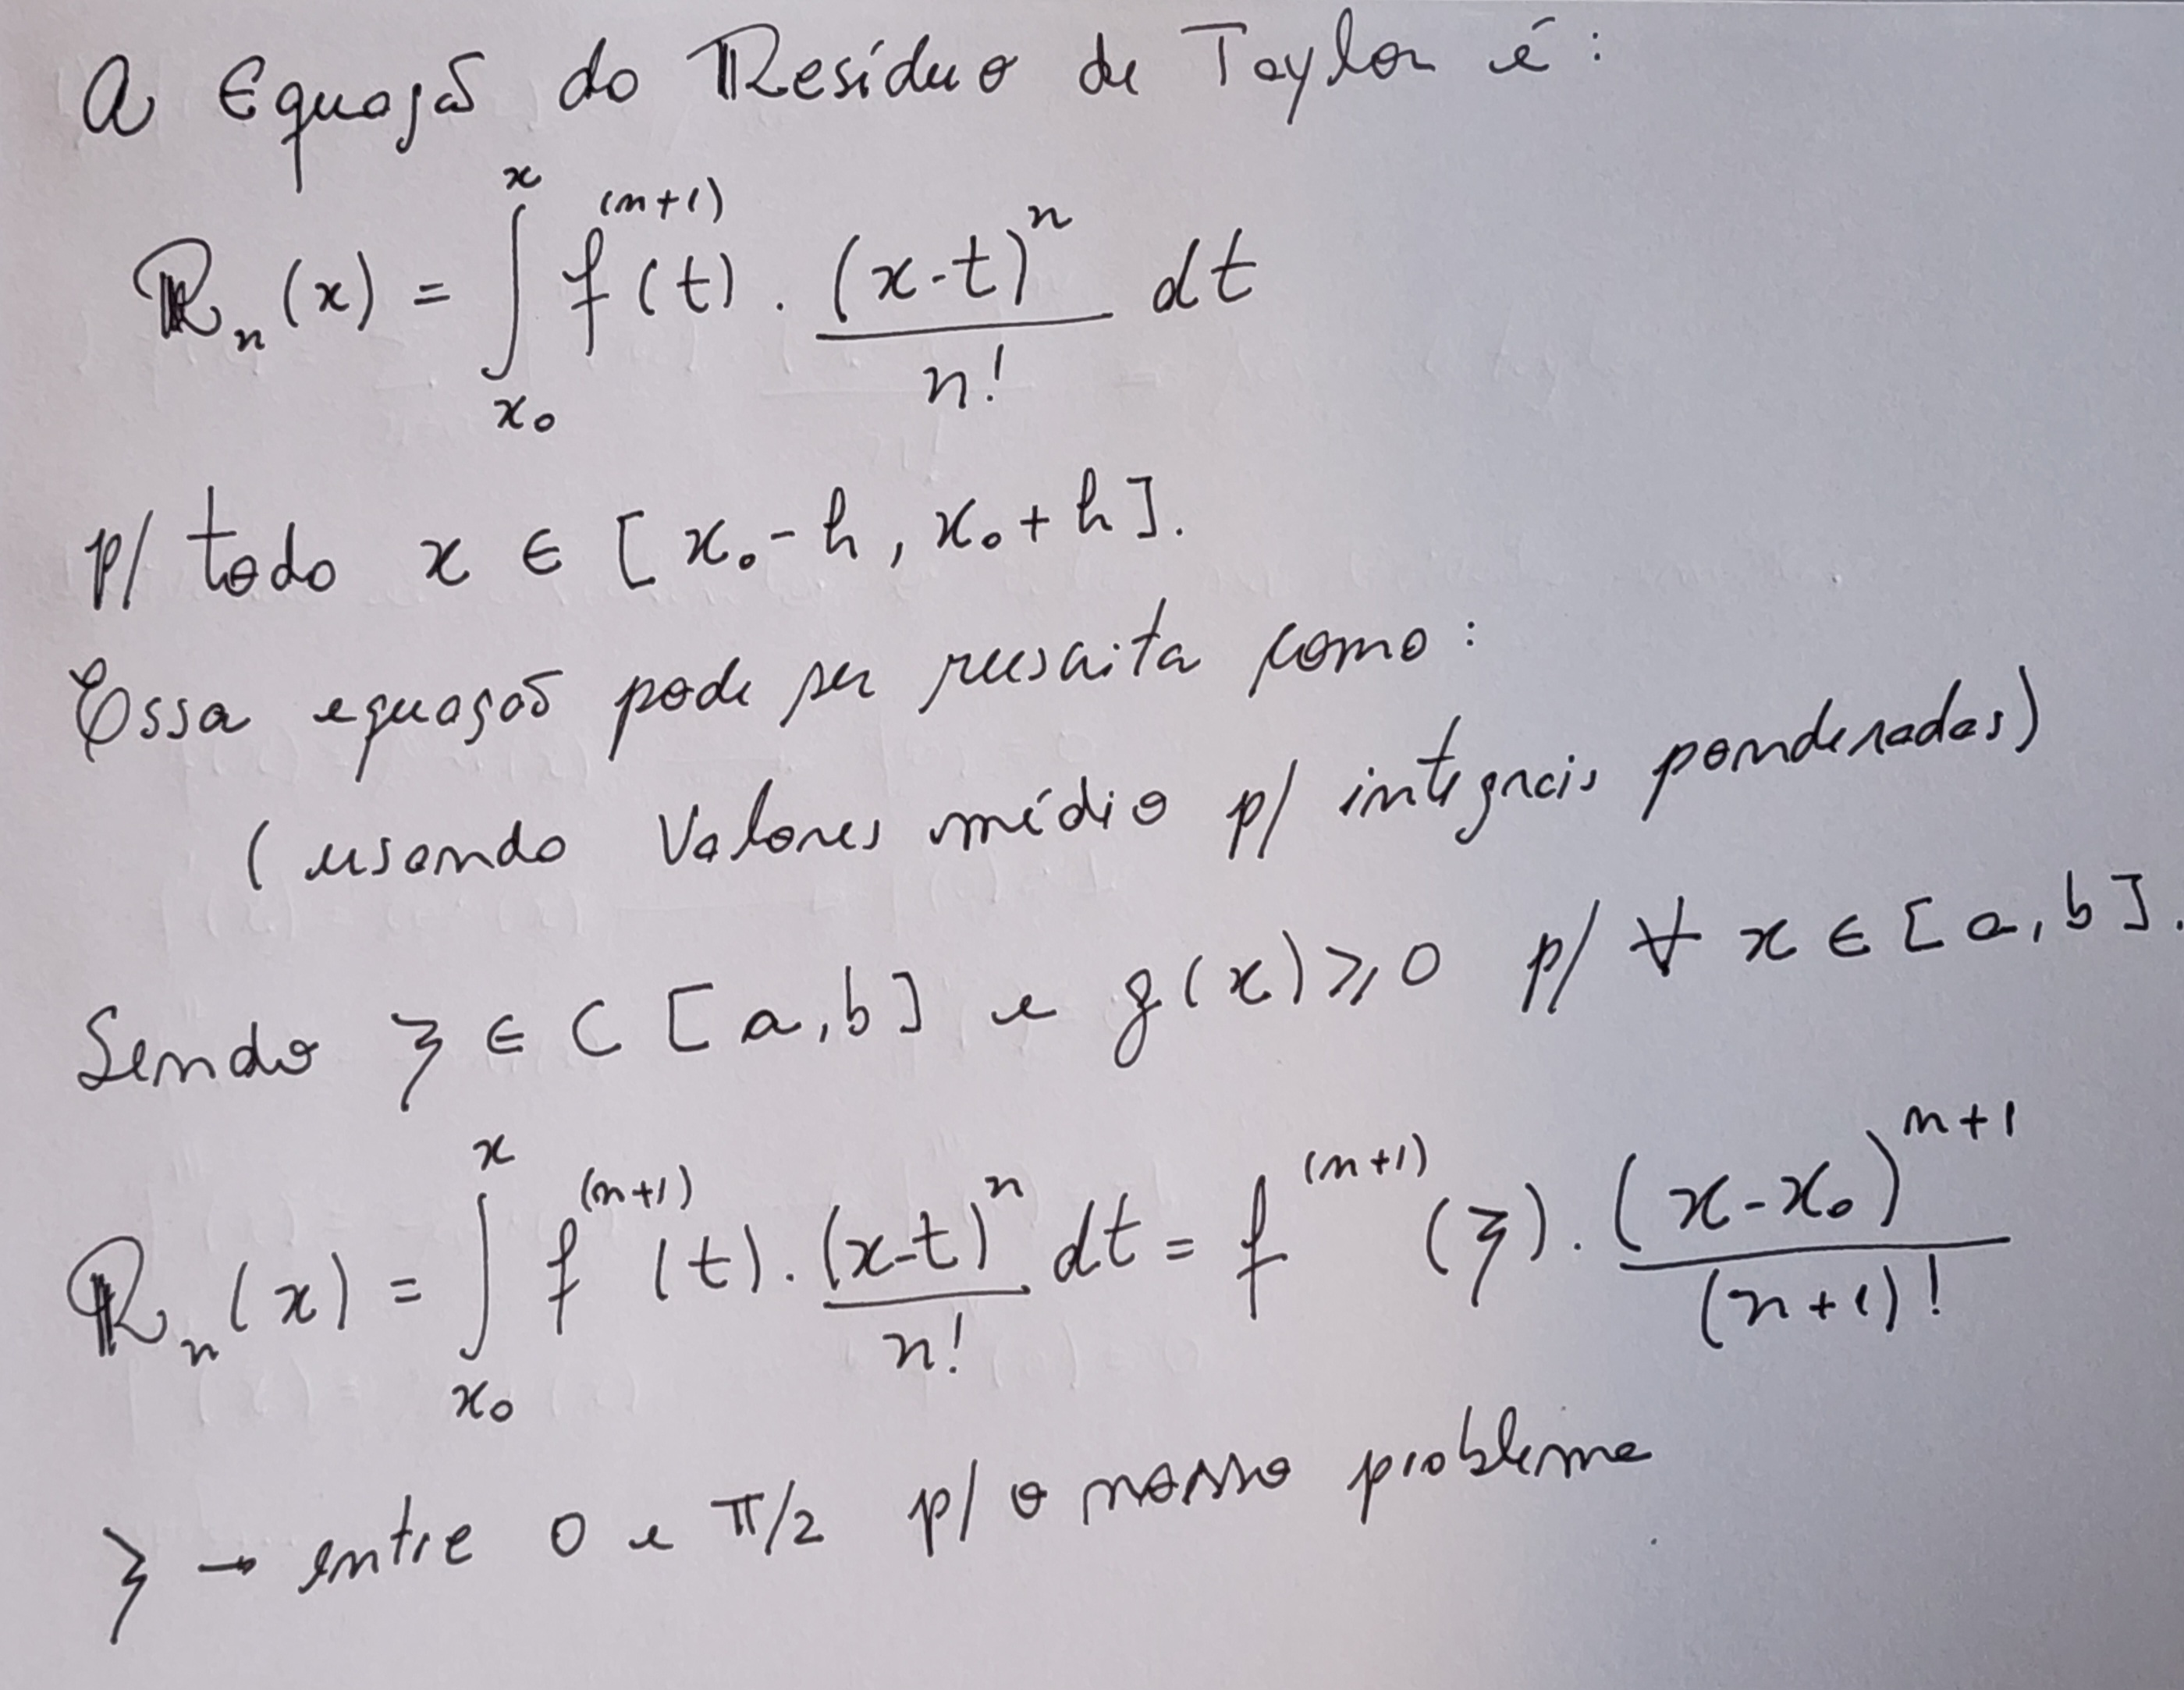
\includegraphics[width=.80\textwidth]{imagens/exercicio3_parte_2}
    \caption{Escrevendo o resíduo}
    \label{fig:lista_exercicio3_parte2}
\end{figure}
Continuando o raciocício e aplicando o resultado do resíduo.
\begin{figure}[H]
    \centering
    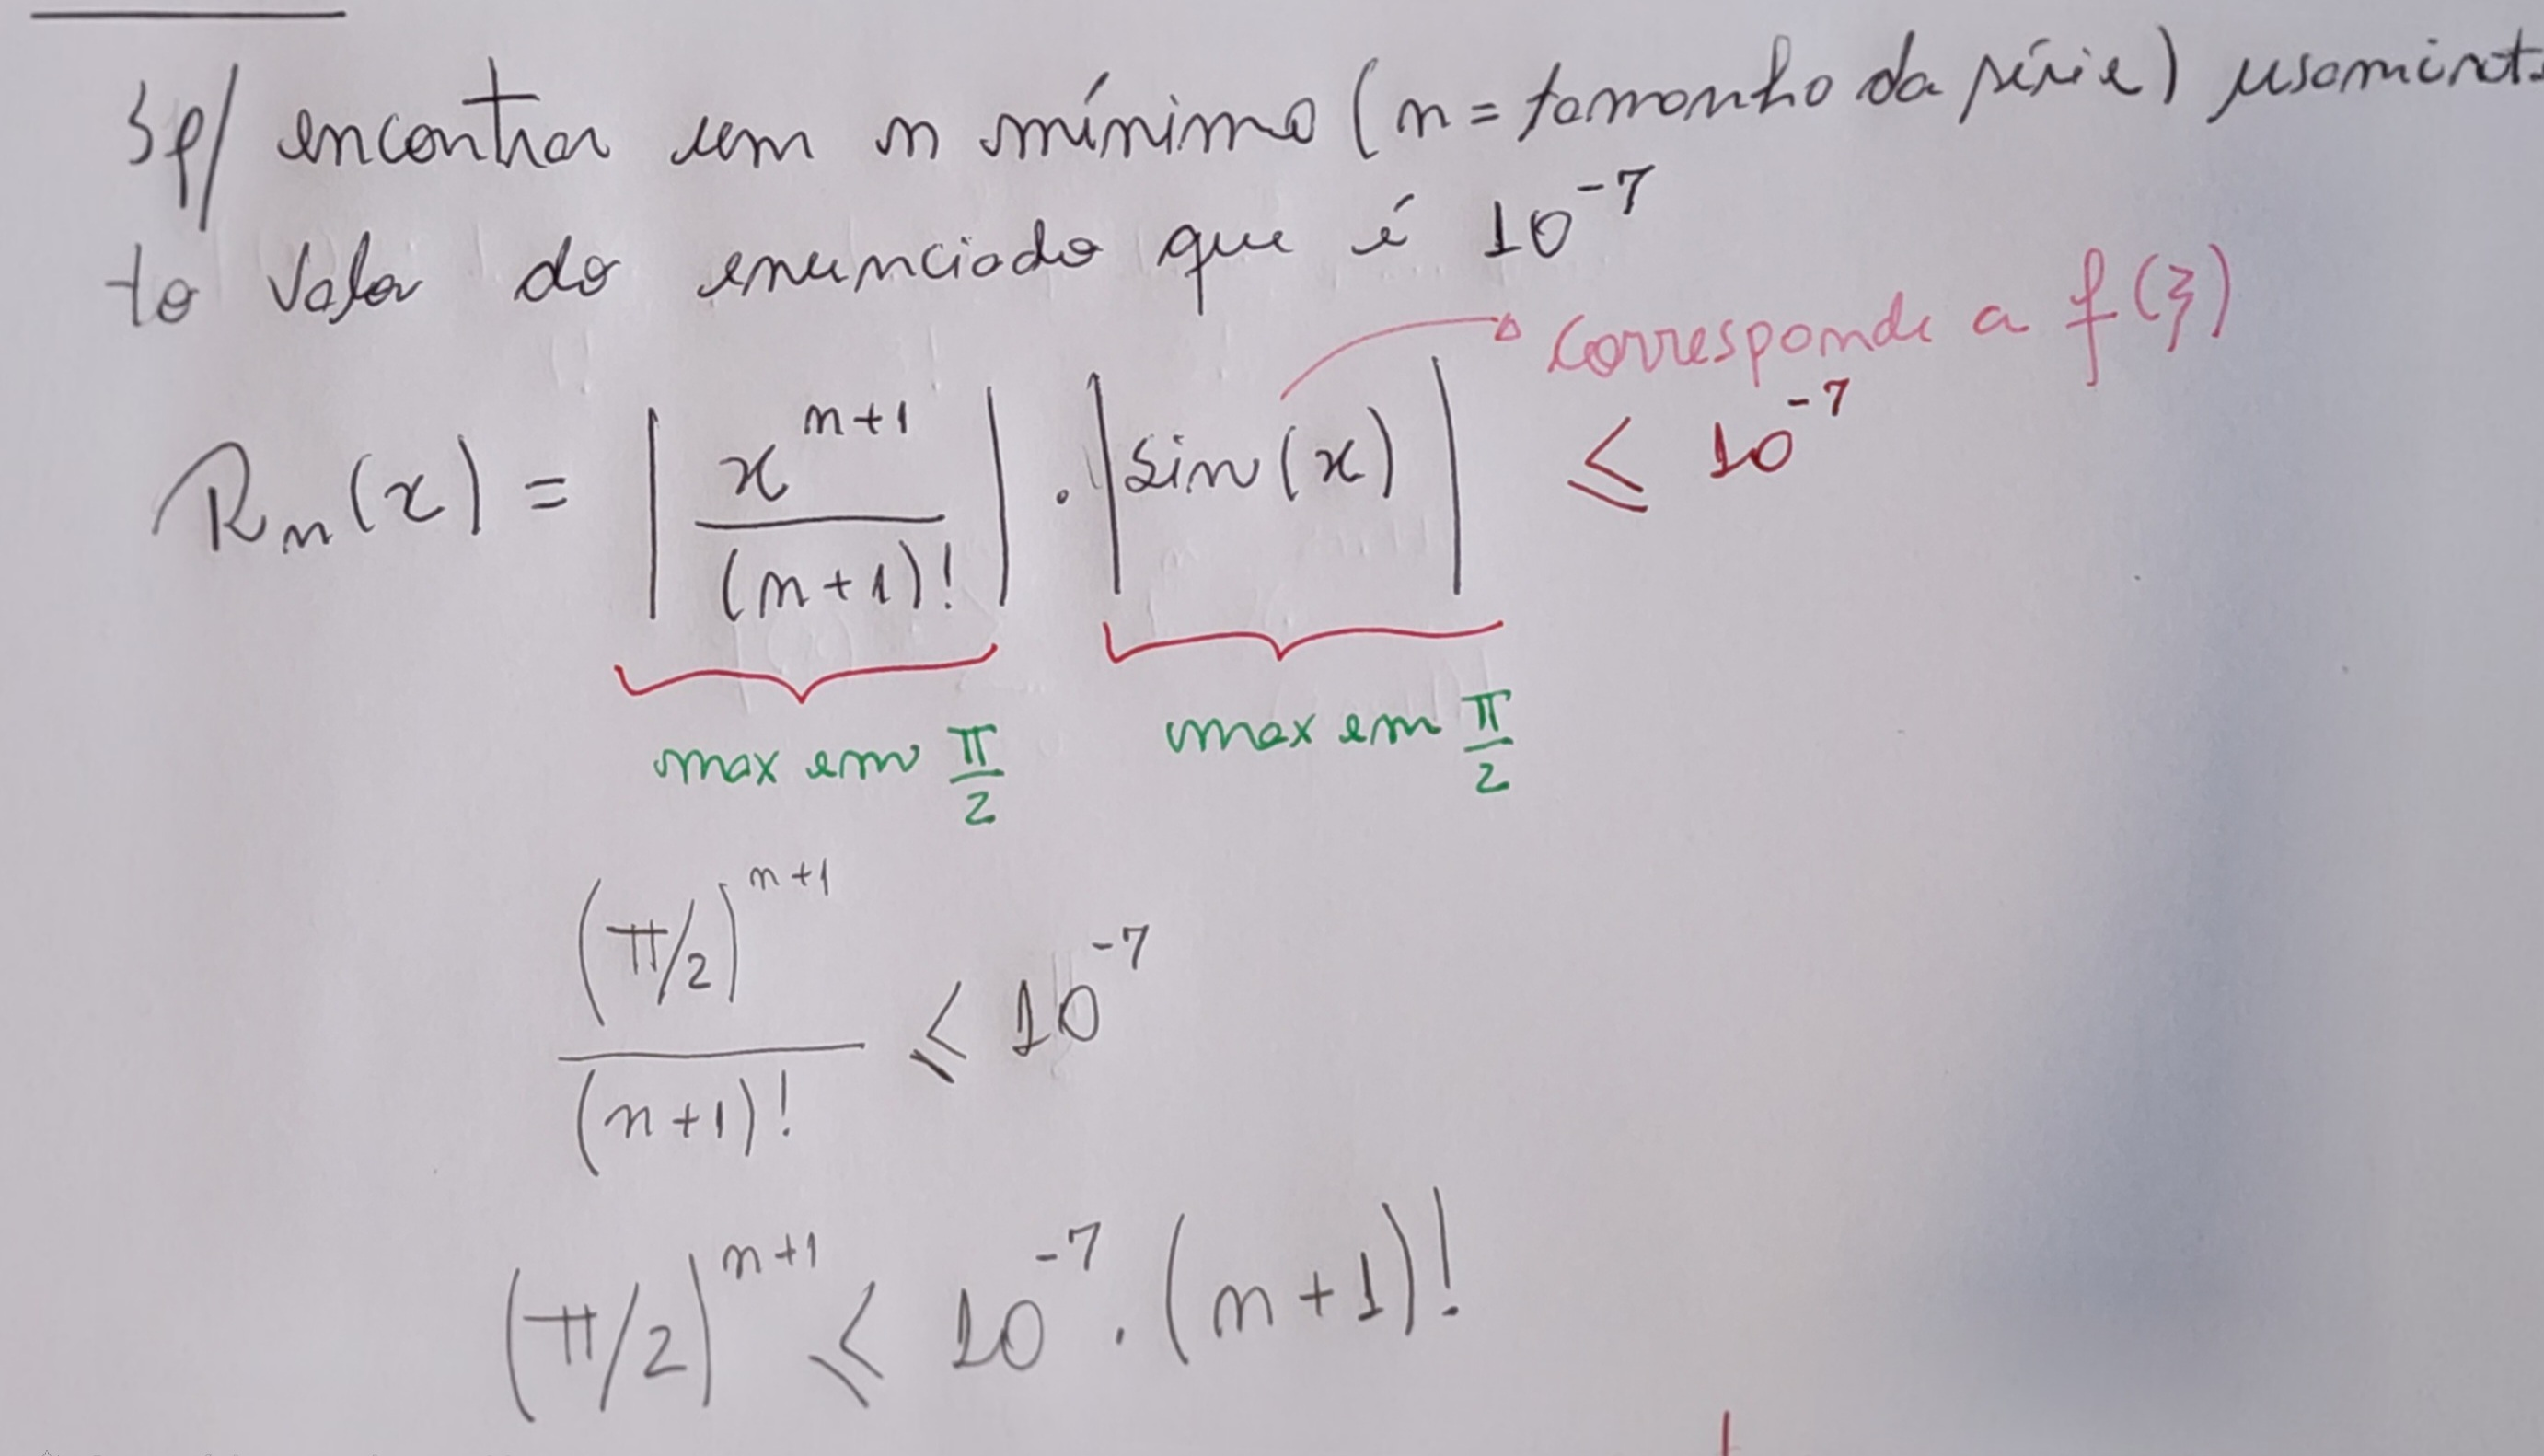
\includegraphics[width=.80\textwidth]{imagens/exercicio3_parte_3}
    \caption{Definindo a equação parar encontrar o valor de N. Essa equação foi testada com valores maiores que 2 e encontramos como verdadeiro o valor 12}
    \label{fig:lista_exercicio3_parte3}
\end{figure}



\newpage
\subsubsection{Imprimir a função na forma de série e usando numpy no python}

Podemos ver nos gráficos da figura \ref{fig:grafico_exe3} que a diferença dos valores entre $-2 \cdot \pi$ a $2 \cdot \pi$ tem basicamente ruído pois está na ordem de $10^{-16}$.
\begin{figure}[H]
    \centering
    \includegraphics[width=1.18\textwidth]{imagens/exercicio3.png}
    \caption{Gráfico da função seno gerada por numpy e $P_2(x)$ e $P_{12}(x)$ e o módulo da diferença de $F(x)$ e $P_{12}(x)$}
    \label{fig:grafico_exe3}
\end{figure}

\newpage

\subsubsection{Realizar os testes}


    \begin{table}[h!]
    \centering
    \caption{Testes do Exercicio 3}
    \begin{tabular}{|c|c|c|c|}
    \toprule
    \textbf{$x$} & \textbf{$f(x)$ (com NumPy)} & \textbf{$f(x)$ (com Taylor)} & \textbf{Diferenca} \\
    \midrule   
    7.0686e+00 & 7.0711e-01 & 7.0711e-01 & 1.1102e-16 \\
                            1.6493e+01 & -7.0711e-01 & -7.0711e-01 & 3.3307e-16 \\
                            3.2201e+01 & 7.0711e-01 & 7.0711e-01 & 6.6613e-16 \\
                            
    \bottomrule
    \end{tabular}
    \end{table}    
    

Vale lembrar que: como temos valores muito próximos em uma subtração essa diferença pode ser um ruido de arredondamento.
Por outro lado como a diferença é menor que $10^{-7}$, o que satisfaz a necessidade da aplicação.\\

\subsubsection{Apresentar o código Python e GnuPlot}
\label{sec:caracteristicas-funcao-sin}
$sin(x)$ é função periódica assim ela é limitando os valores aplicados a $P_{n}(x)$ para valores entre $0$ a $\frac{\pi}{2}$.
Isso está implementado na função \texttt{ajusta\_x\_calculo\_seno} usando as simetrias e periodicidades da função seno.

\lstinputlisting[style=python]{scripts/exercicio3.py}
Código para a geração dos dados em Python.

\newpage
\lstinputlisting[style=gnuplot]{scripts/exercicio3.gnuplot}
Código em GnuPlot para geração dos gráficos do exercício3 baseado nos dados


\newpage





